\chapter{Der konkrete Datentyp Hash-Tabelle und Hash-Verfahren}\label{hash}
In diesem Kapitel soll geklärt werden, was sich hinter dem konkreten Datentypen Hash-Tabelle versteckt und welche Bedeutung das Hashing für diesen hat. Weiterhin soll auf die Hash-Verfahren Doppel-Hashing mit Brents Algorithmus und Kuckucks-Hashing unter Verwendung von Beispielen genauer eingegangen werden.

\section{Der abstrakte Datentyp Wörterbuch}
Abstrakte Datentypen definieren eine Menge von Objekten und darauf ausführbare Operationen \cite[S.~26]{ADSOttWid}, welche mit Hilfe von Programmiersprachen durch konkrete Datentypen implementiert werden. Die möglichst effiziente Implementierung des abstrakten Datentypen Wörterbuch (engl. Dictionary) bezeichnet man auch als Wörterbuchproblem \cite[S.~49]{ADSOttWid}. Zu konkreten Datentypen, die dieses Problem lösen, zählen beispielsweise Listen und Suchbäume. Die Motivation für den konkreten Datentypen Hash-Tabelle ist es, das Wörterbuchproblem zu lösen und dabei für die zu implementierenden Operationen durch direkten Zugriff \cite[S.~235]{ADSWeiWei} bessere Laufzeiten, als bei den vorher genannten konkreten Datentypen zu erreichen. 

Bei den Objekten eines Wörterbuchs handelt es sich um Paare von jeweils einem Schlüssel \(k\) (key) und einem dazugehörigem Wert \(v\) (value). Demnach realisiert ein Wörterbuch eine Abbildung mit endlichem Definitionsbereich \(R\) von Schlüsseln, der auf eine Menge \(V\) von Werten abgebildet wird. Zusätzlich existiert ein Universum \(K\) mit \(R\subseteq{K}\) \cite[S.~191]{ADSOttWid}. 

Die Schnittstelle des abstrakten Datentypen Wörterbuch besteht aus den Operationen Suchen, Einfügen und Entfernen \cite[S.~49]{ADSOttWid}, die folgendermaßen definiert sind:
\begin{itemize}	
\item Einfügen(k,v): Der Datensatz (k,v) wird in die Datenstruktur aufgenommen, sofern \(k\notin{R}\) gilt, andernfalls geschieht nichts.
\item Entfernen(k): Falls ein Datensatz (k,v) in der Datenstruktur existiert, wird dieser aus der Datenstruktur entfernt, andernfalls geschieht nichts.
\item Suchen(k): Gibt einen Wahrheitswert aus, der wahr ist, falls ein Datensatz (k,v) in der Datenstruktur existiert und falsch sonst.
\end{itemize}

In der Lehre zu Hash-Tabellen stehen die Algorithmen zu den Operationen im Mittelpunkt, für die die Werte der Datensätze irrelevant sind. Aus diesem Grund werden im Laufe dieser Arbeit die Werte vernachlässigt, womit ein Datensatz lediglich aus einem Schlüssel besteht\label{novalue}. 

\section{Spezifikation des konkreten Datentypen Hash-Tabelle}
Die \Gls{hashtable} ist ein Array der Länge \(m\), welches mit den Indizes \(0, \dots{},m-1\) versehen ist. Der Begriff Hashing lässt sich zu Deutsch dem Begriff Haschieren, also Zerkleinern, gleichsetzen und beschreibt die Reduktion des Universums \(K\) auf den Definitionsbereich \(R\subseteq{K}\). Durch das Hashing können in Hash-Tabellen beim Einfügen, Löschen und Suchen konstante Laufzeiten erreicht werden, da ein direkter Zugriff auf die Schlüssel ermöglicht wird \cite[S.~235]{ADSWeiWei}.

Soll ein Schlüssel \(k\) in eine Hash-Tabelle eingefügt werden, so muss für \(k\) eine \Gls{hashadress} berechnet werden. Das bedeutet, dass mit Hilfe einer \Gls{hashfunction} \(h: K\to{\{0, \dots{}, m-1\}}\) die Hash-Adresse durch \(h(k)\) berechnet wird, die dem Index entspricht, an dem \(k\) in der Hash-Tabelle eingefügt wird \cite[S.~191]{ADSOttWid}. 

Da die Mächtigkeit des Universums \(|K|\) im Normalfall größer als die Länge \(m\) der Hash-Tabelle ist, kann die Injektivität der Hash-Funktion nicht garantiert werden \cite[S.~191]{ADSOttWid}. Somit existiert mindestens ein Paar von Schlüsseln \(k\) und \(k'\), für die gilt \(h(k)=h(k')\). Man spricht in diesem Fall von einer \Gls{kollisione}\label{kollision} zwischen \(k\) und \(k'\)\cite[S.~235]{ADSWeiWei}.

Eine gute Hash-Funktion zeichnet sich dadurch aus, die Anzahl der Kollisionen zu minimieren, indem alle Schlüssel möglichst gleichmäßig auf die Felder der Hash-Tabelle verteilt werden \cite[S.~193]{ADSOttWid}. Da es sich in der Praxis bei den Schlüsseln nicht immer um natürliche Zahlen handelt, kann außerdem der Einsatz einer Funktion \(code\) nötig werden. Mit Hilfe dieser Funktion lässt sich für einen beliebigen Schlüssel \(k\in{K}\) \(code(k)\in{\mathbb{N}}\) berechnen. Die Hash-Adresse von \(k\) lässt sich also durch \(h(code(k))\) bestimmen \cite[S.~235]{ADSWeiWei}.

Das Datenmodell der Standardbibliothek der Programmiersprache Python schreibt beispielsweise vor, dass ein Schlüssel ein unveränderliches Objekt sein muss. Für jedes unverändliche Objekt gibt es standardmäßig eine Funktion \textit{hash}, die die Speicheradresse des Objekts zurückgibt \cite[ch.~3.4.1.]{PDoc}. Diese Funktion liefert demnach stets eine einzigartige, natürliche Zahl. 

Der Einfachheit halber wird in dieser Arbeit davon ausgegangen, dass es sich bei den Schlüsseln stets um natürliche Zahlen handelt, also der Einsatz einer Funktion \(code\) nicht benötigt wird.

\section{Kollisionsbehandlung beim Einfügen in Hash-Tabellen}
Kommt es beim Einfügen eines Schlüssels zu einer Kollision, wird verhindert, dass der Schlüssel an der berechneten Hash-Adresse eingefügt werden kann. Um dieses Problem zu lösen, gibt es verschiedene Arten der Kollisionsbehandlung. In dieser Hinsicht unterscheidet man zwei Arten von Hashing: das externe und das geschlossene Hashing \cite[S.~239 ff.]{ADSWeiWei}.

Beim externen Hashing (auch Chaining) wird zunächst "jedes Feld der Hash-Tabelle um einen Verweis auf eine verkettete Liste ergänzt" \cite[S.~239]{ADSWeiWei}. Kollidiert ein Schlüssel beim Einfügen, wird dieser, durch Auslagern in die verkettete Liste an der betroffenen Hash-Adresse, in die Hash-Tabelle eingefügt \cite[S.~239]{ADSWeiWei}. Da keine Variante des externen Hashings implementiert werden soll, wird an dieser Stelle auf eine weiterführende Erklärung verzichtet. 

Im Gegensatz zum externen Hashing wird beim geschlossenen Hashing auf externe Strukturen zum Speichern von Schlüsseln verzichtet. Falls es beim geschlossenen Hashing beim Einfügen eines Schlüssels zu einer Kollision kommt, wird versucht, für den einzufügenden Schlüssel eine andere, freie Hash-Adresse zu finden, die durch eine von der Hash-Variante bestimmten Methode ermittelt wird \cite[S.~203]{ADSOttWid}. 

Ferner existiert eine dritte Art von Hash-Verfahren, das perfekte Hashing. Ziel ist es hierbei, eine Hash-Funktion zu finden, bei der keinerlei Kollisionen auftreten, wodurch keine Vorkehrungen zur Kollisionsbehandlung getroffen werden müssen \cite[S.~195]{ADSOttWid}. 

Das geschlossene Hashing ist für diese Arbeit von besonderer Bedeutung, da die beiden Varianten Doppel-Hashing und Kuckucks-Hashing, für welche Aufgaben implementiert werden sollen, zu dieser Kategorie zählen. Im Folgenden werden die Operationen Einfügen, Suchen und Löschen beim geschlossenen Hashing näher beleuchtet.

\section{Einfügen, Suchen und Löschen mit geschlossenem Hashing}\label{loesch}
Entsteht beim Einfügen eines Schlüssels mit dem geschlossenen Hashing eine Kollision, werden solange neue Hash-Adressen bestimmt, bis eine leere Hash-Adresse gefunden wurde, in die der Schlüssel eingefügt wird. Die Folge von Hash-Adressen, die geprüft werden, nennt man \Gls{sondfolg} \cite[S.~203]{ADSOttWid}. Unter Verwendung einer Sondierungsfunktion \(s(j,k)\) mit \(j=0, \dots{},m-1\), ist die Sondierungsfolge definiert durch \((h(k)-s(j,k))\mod{m}\) \cite[S.~204]{ADSOttWid}. Da die Addition für die Anwendung in der Lehre intuitiver als die Subtraktion ist, wird entgegen \cite{ADSOttWid} \((h(k)+s(j,k))\mod{m}\) zur Bestimmung der Sondierungsfolge verwendet.

Das Sondieren beim geschlossenen Hashing hat die Nebenwirkung, dass das Vorgehen bei den Operationen Entfernen, Einfügen und Suchen angepasst werden muss. Zur Veranschaulichung der Beschreibung werden Algorithmen aus \cite[ch.~9.4.4-9.4.5]{ADSWeiWei} verwendet. In diesen Algorithmen wird vorgesehen, dass jedes Feld der Hash-Tabelle einen Status-Attribut hat, welcher entweder \textit{frei}, \textit{belegt} oder \textit{enfernt} ist. Die Notwendigkeit der Status-Attribute wird unter Anderem in diesem Kapitel diskutiert.

Die nachstehende Abbildung zeigt einen Algorithmus für das Einfügen mit geschlossenem Hashing:
\begin{figure}[H]
	\centering
	\includegraphics[width=0.8\textwidth]{Bilder/einfuegen.jpg}
	\caption{Algorithmus zum Einfügen mit geschlossenem Hashing}
	\label{ht_einfuegen}
	\quelle \cite[S.~244]{ADSWeiWei}
\end{figure}

In der Initialisierung des Algorithmus werden die Variablen \textit{j} als Schleifenindex sowie \textit{i} und \textit{index} als erste Hash-Adresse in der Sondierungsfolge des einzufügenden Schlüssels \textit{neuerWert} angelegt. 

Das Sondieren wird in diesem Algorithmus mit Hilfe einer Schleife realisiert (Zeilen 4-8), sobald \(i\) mit einer Hash-Adresse belegt ist, die den Status \(frei\) hat oder den Schlüssel \(neuerWert\) beinhaltet.

Wurde die Schleife abgebrochen, weil der einzufügende Schlüssel bereits Element der Hash-Tabelle ist, so wird in Zeile 10 eine Ausgabe an den Nutzer veranlasst und der Algorithmus beendet. Andernfalls wird der Füllgrad der Hash-Tabelle berechnet (Zeile 11) und falls dieser den Wert \(0.9\) überschreitet, ein \Gls{rehash} durchgeführt und der Algorithmus erneut aufgerufen (Zeilen 12-13). Beim Re-Hashing wird eine längere Hash-Tabelle generiert, in die alle Schlüssel mit einer neuen Hash-Funktion eingefügt werden \cite[S.~244]{ADSWeiWei}. Der Füllgrad einer Hash-Tabelle ist die Anzahl der gespeicherten Schlüssel geteilt durch die Länge der Hash-Tabelle \cite[S.~244]{ADSWeiWei}. 

Ist der Füllgrad der Hash-Tabelle kleiner \(0.9\), so wird der Schlüssel \(neuerWert\) in den Zeilen 16-18 an der Hash-Adresse \(index\) eingefügt und der Status dieser Hash-Adresse auf \textit{belegt} gesetzt.

Da ein Schlüssel nach dem Einfügen an verschiedenen Hash-Adressen in der Hash-Tabelle lokalisiert sein kann, müssen beim Suchen schrittweise die Stellen der Sondierungsfolge des Schlüssels abgeprüft werden, bis entweder der gesuchte Schlüssel oder ein Feld mit dem Status \textit{frei} gefunden wurden \cite[S.~204]{ADSOttWid}. 

Bei dieser Vorgehensweise kann folgendes Problem auftreten: Ein Schlüssel \(k\) wird nach mehrfachem Sondieren eingefügt. Danach löscht man einen anderen Schlüssel \(l\), dessen Hash-Adresse in der Sondierungsfolge von \(k\) vor der Hash-Adresse von \(k\) vorkommt. Wird nun nach dem Schlüssel \(k\) gesucht, bricht die Schleife an der ehemaligen Hash-Adresse von \(l\) ab, da diese den Status \(frei\) hat. Demnach gibt das Suchen fälschlicherweise an, dass der Schlüssel \(k\) nicht in der Hash-Tabelle enthalten ist. Daher müssen beim geschlossenen Hashing in der Hash-Tabelle Felder markiert werden, aus denen ein Schlüssel gelöscht wurde. Zu diesem Zweck gibt es in den Algorithmen von \cite{ADSWeiWei} für Felder den Statuswert \textit{enfernt} \cite[S.~242]{ADSWeiWei}. 

Dementsprechend beschreibt der, in Abbildung~\ref{ht_suchen} dargestellte, Algorithmus das Suchen mit geschlossenem Hashing:
\begin{figure}[H]
	\centering
	\includegraphics[width=0.8\textwidth]{Bilder/suchen.jpg}
	\caption{Algorithmus zum Suchen mit geschlossenem Hashing}
	\label{ht_suchen}
	\quelle \cite[S.~242]{ADSWeiWei}
\end{figure}
Der Algorithmus besteht aus einer Schleife (Zeilen 2-3), die wiederholt wird, bis die Abbruchbedingung aus Zeile 4 erfüllt wird. Dies ist der Fall, wenn der Wert \(i\) eine Hash-Adresse annimmt, die entweder auf ein Feld mit dem gesuchten Schlüssel oder jedoch einem Feld mit dem Status \textit{frei} verweist. Wurde der Schlüssel gefunden, so wird dessen zugehöriger Wert ausgegeben (Zeile 6). Andernfalls wird eine entsprechende Fehlermeldung geliefert (Zeile 7). 

Modifiziert man diesen Algorithmus, wie in Kapitel~\ref{novalue} festgelegt, so, dass die Werte vernachlässigt werden, wird in Zeile 6 stattdessen der Wahrheitswert \textit{wahr} und in Zeile 7 der Wahrheitswert \textit{falsch} ausgegeben.

Der Algorithmus zum Löschen eines Schlüssels unterscheidet sich vom Algorithmus zum Suchen lediglich in der Benennung von Variablen und der Zeile 6. Das Löschen wird folgendermaßen realisiert:
\begin{figure}[H]
	\centering
	\includegraphics[width=0.8\textwidth]{Bilder/loeschen.jpg}
	\caption{Algorithmus zum Löschen mit geschlossenem Hashing}
	\label{ht_loeschen}
	\quelle \cite[S.~243]{ADSWeiWei}
\end{figure}
Beim Löschen wird in Zeile 6 der Status des Feldes, welches den zu löschenden Schlüssel beinhaltet, auf \textit{entfernt} gesetzt. Dadurch wird das Feld für den Algorithmus zum Einfügen als leer betrachtet, da dessen Schleife abbricht, sobald ein Feld auftritt, welches nicht den Status \textit{frei} hat. Für den Algorithmus zum Suchen wiederrum, wird ein mit \textit{entfernt} markiertes Feld als belegt betrachtet, da in diesem Fall die Schleife abbricht, wenn ein Feld aufkommt, dessen Status \textit{frei} ist.

Bei den Operationen mit geschlossenen Hashing ist kein direkter Zugriff mehr möglich, da ein Schlüssel an verschiedenen Hash-Adressen lokalisiert sein kann. Aus diesem Grund sind die Laufzeiten vom Füllgrad der entsprechenden Hash-Tabelle abhängig. Je höher der Füllgrad, desto mehr Schritte werden durchschnittlich bei der Anwendung der Operationen benötigt \cite[S.~211]{ADSOttWid}.

\section{Das Doppel-Hashing mit Brents Algorithmus}\label{brent}
Eine Variante des geschlossenen Hashings ist das Doppel-Hashing. Bei dieser Variante wird neben der Hash-Funktion \(h(k)\) eine zweite Hash-Funktion \(h'(k)\) verwendet, um eine Schrittweite zu berechnen \cite[S.~247]{ADSWeiWei}. Aus den beiden Hash-Funktionen lässt sich die Sondierungsfunktion \(s(j,k) = h(k)+j\cdot{}h'(k)\) mit \(j=0, \dots{},m-1\) bilden \cite[S.~275]{algoeinf}. Die Sondierungsfolge wird mit Hilfe der Sondierungsfunktion bestimmt und findet bei der Ausführung der Operationen, wie im vorherigen Unterkapitel beschrieben, Anwendung.

Modifiziert man das Doppel-Hashing unter Verwendung von Brents Algorithmus, ist folgender Algorithmus für das Einfügen von Schlüsseln anzuwenden:
\begin{figure}[H]
	\centering
	\includegraphics[width=0.8\textwidth]{Bilder/einfuegen_brent.jpg}
	\caption{Algorithmus zum Einfügen mit Doppel-Hashing mit Brents Algorithmus}
	\label{ht_einfuegen_brent}
	\quelle \cite[S.~250]{ADSWeiWei}
\end{figure}
In einer Schleife wird in den Zeilen 2-9 die Sondierungsfolge des einzufügenden Schlüssels durchlaufen, bis eine Hash-Adresse erreicht wird, die nicht den Status \textit{belegt} hat. Die Variable \textit{i} dient dem Speichern der Hash-Adresse, die abgeprüft wird.

Innerhalb der Schleife wird sowohl die nächste Hash-Adresse des einzufügenden Schlüssels (Zeile 3), als auch die nächste Hash-Adresse des Schlüssels berechnet, der an der Hash-Adresse \textit{i} gespeichert ist (Zeile 4). Die Hash-Adressen werden in den Variablen \textit{neufolgt} und \textit{altfolgt} gespeichert. Hat die Hash-Adresse \textit{neufolgt} den Status \textit{frei} und die Hash-Adresse \textit{altfolgt} den Status \textit{belegt}, so wird die Schleife erneut ausgeführt, nachdem \textit{i} der Wert von \textit{neufolgt} zugewiesen wurde (Zeile 6). Andernfalls wird der an der Hash-Adresse \textit{i} gespeicherte Schlüssel gelöscht und an der Hash-Adresse \textit{altfolgt} eingefügt (Zeile 7). Dies führt außerdem zum Abbruch der Schleife, da der Status der Hash-Adresse \textit{i} auf \textit{entfernt} gesetzt wurde (Zeile 9).

Ist die Schleife beendet, wird der Schlüssel \(neuerWert\) an der Hash-Adresse \textit{i} eingefügt (Zeilen 10-12). 

\section{Beispiel zum Doppel-Hashing mit Brents Algorithmus}\label{examplebrent}
Um den Algorithmus zum Einfügen zu verbildlichen, folgt nun ein Beispiel aus \cite[S.~214]{ADSOttWid}, welches in Kapitel~\ref{implement} mit Hilfe des autotools nachgestellt wird: 

Betrachtet wird eine leere Hash-Tabelle \(ht\) der Länge \(m=7\), in die nacheinander die Schlüssel 12, 53, 5, 15, 2, 19 und 6 eingefügt werden. Zusätzlich zum ursprünglichen Beispiel wird zum Schluss der Schlüssel 6 eingefügt. Das Einfügen erfolgt mit Hilfe der Hash-Funktionen \(h(k)=k\mod{7}\) und \(h'(k)=1+k\mod{5}\). 

Zunächst werden die Funktionswerte der beiden Hash-Funktionen für jeden Schlüssel berechnet und in Tabelle~\ref{tab:hashwerte_b} dargestellt:
\begin{table}[H]
	\centering
	\begin{tabular}{|c|c|c|}
		\hline
		\(k\) & \(h(k)\) & \(h'(k)\) \\ \hline
		12 & 5 & 3 \\
		53 & 4 & 4 \\
		5 & 5 & 1 \\
		15 & 1 & 1 \\
		2 & 2 & 3 \\
		19 & 5 & 5 \\
		6 & 6 & 2 \\ \hline
	\end{tabular}
	\caption{Hash-Adressen für die einzufügenden Schlüssel beim Doppel-Hashing mit Brents Algorithmus}
	\label{tab:hashwerte_b}
\end{table}
Für einen Schlüssel \(k\) ist demnach \(h(k)\) das erste Glied der Sondierungsfolge und \(h'(k)\) die Schrittweite, welche auf ein Glied der Sondierungsfolge addiert wird, um das nächste Glied zu berechnen.

Die Schlüssel 12 und 53 werden kollisionsfrei an den Hash-Adressen 5 und 4 eingefügt. Die Abbildung~\ref{brent_bsp_1} zeigt die Hash-Tabelle \(ht\) nach dem Einfügen der beiden Schlüssel:
\begin{figure}[H]
	\centering
	\begin{tikzpicture}[scale=1.4]
	\foreach \x in {1,2,...,7} {
		\draw (\x,0) rectangle (\x+1,1);
		\tikzmath{int \y; \y=\x-1;}
		\node at (\x+0.5,-0.2) {\scriptsize \y};
	}
	\node at (0.5,0.5) {ht:};
	\node at (5.5,0.5) {\color{purple}53};
	\node at (6.5,0.5) {\color{purple}12};
	\end{tikzpicture}
	\caption{\(ht\) nach dem Einfügen der Schlüssel 12 und 53}
	\label{brent_bsp_1}
\end{figure}
Als Nächstes wird der Schlüssel \(k=5\) eingefügt, wobei es zu einer Kollision bei der Hash-Adresse 5 mit dem Schlüssel \(k'=12\) kommt. Man betrachtet die nächsten Hash-Adressen \(p\) und \(p'\) in den Sondierungsfolgen der beiden Schlüssel. Diese berechnen sich durch \(p=(5+1)\mod{7}=6\) und \(p'=(5+3)\mod{7}=1\). Da die Hash-Adresse \(p=6\) frei ist, wird der Schlüssel 5 dort eingefügt, woraus folgende in Abbildung~\ref{brent_bsp_2} dargestellte Hash-Tabelle \(ht\) entsteht:
\begin{figure}[H]
	\centering
	\begin{tikzpicture}[scale=1.4]
	\foreach \x in {1,2,...,7} {
		\draw (\x,0) rectangle (\x+1,1);
		\tikzmath{int \y; \y=\x-1;}
		\node at (\x+0.5,-0.2) {\scriptsize \y};
	}
	\node at (0.5,0.5) {ht:};
	\node at (5.5,0.5) {53};
	\node at (6.5,0.5) {12};
	\node at (7.5,0.5) {\color{purple}5};
	\end{tikzpicture}
	\caption{\(ht\) nach dem Einfügen des Schlüssels 5}
	\label{brent_bsp_2}
\end{figure}
Die Schlüssel 15 und 2 werden kollisionsfrei an den Hash-Adressen 1 und 2 eingefügt. Die Operationen liefern die Hash-Tabelle \(ht\) in Abbildung~\ref{brent_bsp_3}:
\begin{figure}[H]
	\centering
	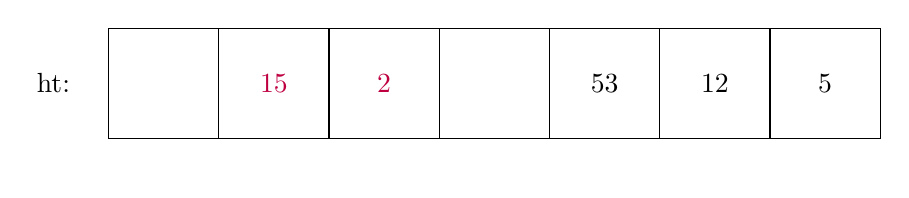
\begin{tikzpicture}[scale=1.4]
	\foreach \x in {1,2,...,7} {
		\draw (\x,0) rectangle (\x+1,1);
		\tikzmath{int \y; \y=\x-1;}
		\node at (\x+0.5,-0.2) {\scriptsize \y};
	}
	\node at (0.5,0.5) {ht:};
	\node at (2.5,0.5) {\color{purple}15};
	\node at (3.5,0.5) {\color{purple}2};
	\node at (5.5,0.5) {53};
	\node at (6.5,0.5) {12};
	\node at (7.5,0.5) {5};
	\end{tikzpicture}
	\caption{\(ht\) nach dem Einfügen der Schlüssel 15 und 2}
	\label{brent_bsp_3}
\end{figure}
Nun wird der Schlüssel \(k=19\) eingefügt. Dabei kommt es zu einer Kollision an der Hash-Adresse 5 mit dem Schlüssel \(k'=12\). Anschließend werden die Hash-Adressen \(p=(5+5)\mod{7}=3\) und \(p'=(5+3)\mod{7}=1\) berechnet. Die Hash-Adresse \(p=3\) ist frei, also wird der Schlüssel 19 dort eingefügt, wodurch sich die nachstehende Hash-Tabelle \(ht\) ergibt (Abbildung~\ref{brent_bsp_4}):
\begin{figure}[H]
	\centering
	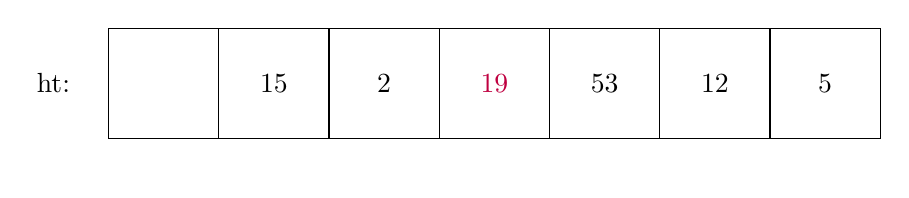
\begin{tikzpicture}[scale=1.4]
	\foreach \x in {1,2,...,7} {
		\draw (\x,0) rectangle (\x+1,1);
		\tikzmath{int \y; \y=\x-1;}
		\node at (\x+0.5,-0.2) {\scriptsize \y};
	}
	\node at (0.5,0.5) {ht:};
	\node at (2.5,0.5) {15};
	\node at (3.5,0.5) {2};
	\node at (4.5,0.5) {\color{purple}19};
	\node at (5.5,0.5) {53};
	\node at (6.5,0.5) {12};
	\node at (7.5,0.5) {5};
	\end{tikzpicture}
	\caption{\(ht\) nach dem Einfügen des Schlüssels 19}
	\label{brent_bsp_4}
\end{figure}
Bei der letzten Operation, dem Einfügen des Schlüssels 6, kommt es mit dem Schlüssel 5 zu einer Kollision an der Hash-Adresse 6. Die nächsten Hash-Adressen in den Sondierungsfolgen der beiden Schlüssel sind \(p=(6+2)\mod{7}=1\) und \(p'=(6+1)\mod{7}=0\). Da \(p\) belegt und \(p'\) frei ist, wird der Schlüssel 5 auf die Hash-Adresse \(p'=0\) verschoben und der Schlüssel 6 an der dadurch frei gewordenen Hash-Adresse 6 eingefügt. In Abbildung~\ref{brent_bsp_5} wird die Hash-Tabelle \(ht\) nach Durchführung aller Operation dargestellt:
\begin{figure}[H]
	\centering
	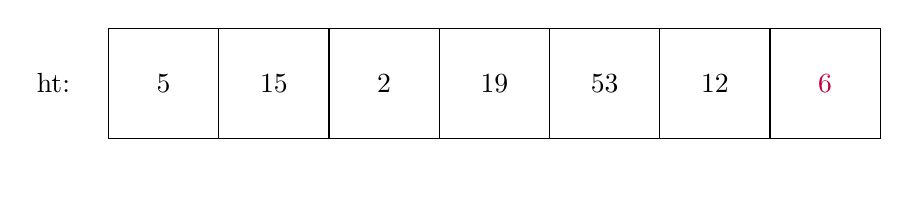
\begin{tikzpicture}[scale=1.4]
	\foreach \x in {1,2,...,7} {
		\draw (\x,0) rectangle (\x+1,1);
		\tikzmath{int \y; \y=\x-1;}
		\node at (\x+0.5,-0.2) {\scriptsize \y};
	}
	\node at (0.5,0.5) {ht:};
	\node at (1.5,0.5) {5};
	\node at (2.5,0.5) {15};
	\node at (3.5,0.5) {2};
	\node at (4.5,0.5) {19};
	\node at (5.5,0.5) {53};
	\node at (6.5,0.5) {12};
	\node at (7.5,0.5) {\color{purple}6};
	\end{tikzpicture}
	\caption{\(ht\) nach dem Einfügen des Schlüssels 6}
	\label{brent_bsp_5}
\end{figure}

\section{Das Kuckucks-Hashing}\label{kuckuck}
Das Kuckucks-Hashing ist ein weiterer Ansatz, um Kollisionen beim Hashing zu lösen, welcher beim Suchen zu einer konstanten Worst Case Laufzeit führt \cite[S.~22]{ADScuckoo}. Außergewöhnlich ist bei dieser Variante, dass zwei Hash-Tabellen \(T_{1}\) und \(T_{2}\) der Länge \(m\) mit zwei Hash-Funktionen \(h_{1}\) und \(h_{2}\) benutzt werden. Für jeden Schlüssel \(x\in{R}\) gilt entweder \(t_{1}[h_{1}(x)]=x\) oder \(t_{2}[h_{2}(x)]=x\). \\ 
Folgender Algorithmus beschreibt nach \cite[S.~3]{ADScuckoo} das Suchen beim Kuckucks-Hashing:
\newpage
\begin{lstlisting} [caption={Algorithmus zum Suchen mit Kuckucks-Hashing}]
function lookup(x)
	return @/\(T_{1}[h_{1}(x)]\)/@ = x @/\(\vee\)/@ @/\(T_{2}[h_{2}(x)]\)/@ = x
end
\end{lstlisting}
Es werden maximal zwei Hash-Adressen für den gesuchten Schlüssel abgeprüft, wodurch beim Suchen eine konstante Laufzeit zustande kommt \cite[S.~3]{ADScuckoo}. 

Beim Löschen eines Schlüssels wird auf die gleiche Weise vorgegangen: Die beiden relevanten Adressen werden auf Existenz des Schlüssels übergeprüft und falls der Schlüssel gefunden wurde, so wird er aus der entsprechenden Hash-Tabelle gelöscht \cite[S.~3]{ADScuckoo}. 

Das Verhalten beim Einfügen ist, was dieser Variante ihren Namen gibt: Kommt es beim Einfügen in die erste Hash-Tabelle zu einer Kollision, wird der Schlüssel, der die entsprechende Hash-Adresse belegt, in ein anderes „Nest“ (Feld in der zweiten Hash-Tabelle) verdrängt \cite[S.~4]{ADScuckoo}. 

Soll beispielsweise ein Schlüssel \(x\) in die Hash-Tabellen \(T_{1}\) und \(T_{2}\) mit den Hash-Funktionen \(h_{1}\) und \(h_{2}\) einfügt werden, wird \(x\) an der Hash-Adresse \(h_{1}(x)\) eingefügt. Falls die Hash-Adresse vor dem Einfügen durch einen anderen Schlüssel belegt war, wird dieser in die andere Hash-Tabelle \(T_{2}\) eingefügt. Auf diese Weise werden abwechselnd Schlüssel in den beiden Hash-Tabellen eingefügt, bis keine Kollision mehr auftritt \cite[S.~4]{ADScuckoo}. 
\newpage
Das Einfügen mit dem Kuckucks-Hashing wird durch den nachstehenden Algorithmus von \cite[S.~5]{ADScuckoo} umgesetzt:
\begin{lstlisting} [caption={Algorithmus zum Einfügen mit Kuckucks-Hashing}]
procedure insert(x)
	if lookup(x) then return
	loop MaxLoop times
		x @/\(\leftrightarrow\)/@ @/\(T_{1}[h_{1}(x)]\)/@
		if x = @/\(\bot\)/@ then return
		x @/\(\leftrightarrow\)/@ @/\(T_{2}[h_{2}(x)]\)/@
		if x = @/\(\bot\)/@ then return
	end loop
	rehash(); insert(x)
end
\end{lstlisting}
Der zweistellige Operator \(\leftrightarrow\) bewirkt den Tausch zweier Variablen und der nullstellige Operator \(\bot\) ("Bottom") steht für einen "leeren Eintrag" \cite[S.~73]{ADSWeiWei}. In Zeile 2 wird die Such-Operation auf den einzufügenden Schlüssel \(x\) ausgeführt, um sicher zu gehen, dass dieser nicht bereits in einer der beiden Tabellen vorhanden ist. Wird \(x\) nicht gefunden, so beginnt in Zeile 3 eine Schleife, die maximal \(MaxLoop\) mal wiederholt wird. Die externe Variable \(MaxLoop\) soll verhindern, dass der Algorithmus nicht terminiert \cite[S.~4]{ADScuckoo}. 

In Zeile 4 wird der Schlüssel \(x\) mit dem Wert \(T_{1}[h_{1}(x)]\) getauscht. Folglich wird \(x\) an der Hash-Adresse \(h_{1}(x)\) in \(T_{1}\) eingefügt und mit dem Wert belegt, den das Feld \(h_{1}(x)\) vor dem Einfügen hatte. Wenn \(x\) gleich dem leeren Eintrag \(\bot\) ist (Zeile 5), also in Zeile 4 kollisionsfrei eingefügt wurde, wird der Algorithmus beendet. Die gleiche Prozedur wird in den Zeilen 6-7 für die zweite Hash-Tabelle \(T_{2}\) durchgeführt. 

Wurde die Schleife durch Eintreten der Abbruchbedingung beendet, so wird ein Re-Hashing durchgeführt und danach die Einfüge-Operation erneut aufgerufen. Re-Hashing bedeutet das Vergrößern der Hash-Tabellen und Einfügen der Schlüssel mit neuen Hash-Funktionen \cite[S.~4]{ADScuckoo}.

\section{Beispiel zum Kuckucks-Hashing}\label{examplecuck}
Es folgt ein Bespiel zur Veranschaulichung der Vorgehensweise beim Einfügen mit dem Kuckucks-Hashing, welches in Kapitel~\ref{implement} mit Hilfe des autotools nachgestellt wird: 

Betrachtet werden zwei leere Hash-Tabellen \(ht_{1}\) und \(ht_{2}\) der Länge \(m=5\) mit den beiden Hash-Funktionen \(h_{1}(k)=k\mod{5}\) und \(h_{2}(k)=k\mod{7}\mod{5}\). Es werden nacheinander die Schlüssel 1, 7, 13, 11, 3 und 6 eingefügt. 

Um das Einfügen zu erleichtern, bietet es sich an, vorher für jeden Schlüssel die Hash-Adressen mit den beiden Hash-Funktionen zu berechnen. In folgender Tabelle~\ref{tab:hashwerte_k} sind jene Hash-Adressen dargestellt: 
\begin{table}[H]
	\centering
	\begin{tabular}{|c|c|c|}
		\hline
		k & \(h_{1}(k)\) & \(h_{2}(k)\) \\ \hline
		1 & 1 & 1 \\
		7 & 2 & 0 \\
		13 & 3 & 1 \\
		11 & 1 & 4 \\
		3 & 3 & 3 \\
		6 & 1 & 1 \\ \hline
	\end{tabular}
	\caption{Hash-Adressen für die einzufügenden Schlüssel beim Kuckucks-Hashing}
 	\label{tab:hashwerte_k}
\end{table}
Die Einfüge-Operationen werden nacheinander beschrieben und anhand von Abbildungen verbildlicht. Darin befinden sich, mit Buchstaben beschriftete, Pfeile, die in der Beschreibung zu den entsprechenden Operationen referenziert werden. Da es beim Einfügen mit dem Kuckucks-Hashing zum Verschieben mehrerer Schlüssel kommen kann, sollen die Pfeile dazu dienen, die Übersicht zu erhalten. 

Das Einfügen der ersten drei Schlüssel \textit{1} in Schritt A, \textit{7} in Schritt B und \textit{13} in Schritt C erfolgt ohne Kollision und resultiert in den in Abbildung~\ref{cuckoo_bsp_1} dargestellten Hash-Tabellen:
\begin{figure}[H]
	\centering
	\begin{tikzpicture}[scale=1]
	\foreach \x in {1,2,3,4,5} {
		\tikzmath{int \y; \y=\x-1;}
		\draw (0,\x) rectangle (1,\x+1);
		\node at (-0.2,\x+0.5) {\scriptsize \y};
		\draw (4,\x) rectangle (5,\x+1);
		\node at (5.2,\x+0.5) {\scriptsize \y};
	}
	\node at (0.5,0.5) {\(ht_{1}\)};
	\node at (4.5,0.5) {\(ht_{2}\)};
	\node at (0.5,2.5) {\color{purple}1};
	\node at (0.5,3.5) {\color{purple}7};
	\node at (0.5,4.5) {\color{purple}13};
	\draw[->, line width=1.2pt] (-1.5,2.5) -- (-.4,2.5);
	\draw[->, line width=1.2pt] (-1.5,3.5) -- (-.4,3.5);
	\draw[->, line width=1.2pt] (-1.5,4.5) -- (-.4,4.5);
	\node at (-1.9,2.5) {(A)};
	\node at (-1.9,3.5) {(B)};
	\node at (-1.9,4.5) {(C)};
	\end{tikzpicture}
	\caption{\(ht_{1}\) und \(ht_{2}\) nach dem Einfügen der Schlüssel 1, 7 und 13}
	\label{cuckoo_bsp_1}
\end{figure}
Beim Einfügen des Schlüssels \textit{11} kommt es zu einer Kollision, da die Hash-Adresse \(h_{1}(11)=1\) in \(ht_{1}\) bereits durch den Schlüssel \textit{1} belegt ist. Zunächst wird der Schlüssel \textit{11}  in Schritt A  an der Hash-Adresse 1 in \(ht_{1}\) eingefügt. Danach wird der Schlüssel \textit{1} in Schritt B auf die Hash-Adresse 1 in \(ht_{2}\) verschoben. Das Einfügen des Schlüssels \textit{1} ist kollisionsfrei, wodurch die Operation beendet wird und folgende Hash-Tabellen aus Abbildung~\ref{cuckoo_bsp_2} entstehen:
\begin{figure}[H]
	\centering
	\begin{tikzpicture}[scale=1]
	\foreach \x in {1,2,3,4,5} {
		\tikzmath{int \y; \y=\x-1;}
		\draw (0,\x) rectangle (1,\x+1);
		\node at (-0.2,\x+0.5) {\scriptsize \y};
		\draw (4,\x) rectangle (5,\x+1);
		\node at (5.2,\x+0.5) {\scriptsize \y};
	}
	\node at (0.5,0.5) {\(ht_{1}\)};
	\node at (4.5,0.5) {\(ht_{2}\)};
	\node at (0.5,2.5) {\color{purple}11};
	\node at (0.5,3.5) {7};
	\node at (0.5,4.5) {13};
	\node at (4.5,2.5) {1};
	\draw[->, line width=1.2pt] (-1.5,2.5) -- (-.4,2.5);
	\draw[->, line width=1.2pt] (1.9,2.5) -- (3.75,2.5);
	\node at (-1.9,2.5) {(A)};
	\node at (1.5,2.5) {(B)};
	\end{tikzpicture}
	\caption{\(ht_{1}\) und \(ht_{2}\) nach dem Einfügen des Schlüssels 11}
	\label{cuckoo_bsp_2}
\end{figure}
Als nächstes wird der Schlüssel \textit{3} in Schritt A an Hash-Adresse 3 in \(ht_{1}\) eingefügt. Da dieses Feld von Schlüssel \textit{13} besetzt war, wird dieser in Schritt B an die Hash-Adresse 1 in \(ht_{2}\) verschoben. Dieses Feld war durch den Schlüssel \textit{1} belegt, welcher in Schritt C in \(ht_{1}\) an die Hash-Adresse 1 eingefügt wird. Dadurch wird der Schlüssel \textit{11} in \(ht_{2}\) verdrängt. Dieser wird in Schritt D ohne Kollision an der Hash-Adresse 4 eingefügt. Abbildung~\ref{cuckoo_bsp_3} stellt die Hash-Tabellen nach dem Abschluss der Einfüge-Operation dar:
\begin{figure}[H]
	\centering
	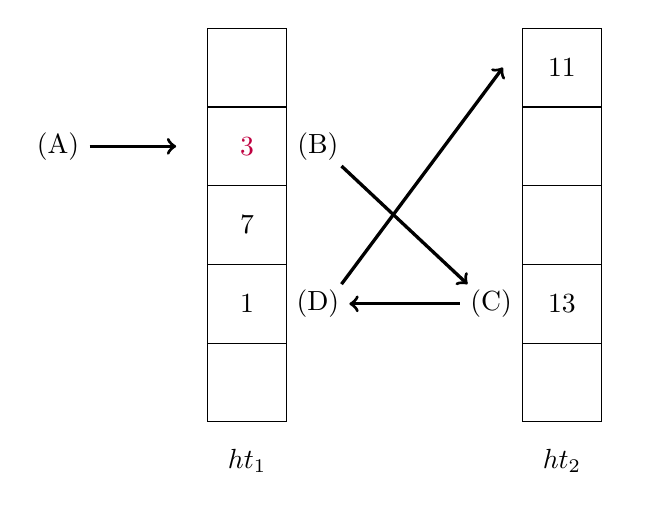
\begin{tikzpicture}[scale=1]
	\foreach \x in {1,2,3,4,5} {
		\tikzmath{int \y; \y=\x-1;}
		\draw (0,\x) rectangle (1,\x+1);
		\node at (-0.2,\x+0.5) {\scriptsize \y};
		\draw (4,\x) rectangle (5,\x+1);
		\node at (5.2,\x+0.5) {\scriptsize \y};
	}
	\node at (0.5,0.5) {\(ht_{1}\)};
	\node at (4.5,0.5) {\(ht_{2}\)};
	\node at (0.5,2.5) {1};
	\node at (0.5,3.5) {7};
	\node at (0.5,4.5) {\color{purple}3};
	\node at (4.5,5.5) {11};
	\node at (4.5,2.5) {13};
	\draw[->, line width=1.2pt] (-1.5,4.5) -- (-.4,4.5);
	\draw[->, line width=1.2pt] (1.7,4.25) -- (3.3,2.75);
	\draw[->, line width=1.2pt] (3.2,2.5) -- (1.8,2.5);
	\draw[->, line width=1.2pt] (1.7,2.75) -- (3.75,5.5);
	\node at (-1.9,4.5) {(A)};
	\node at (1.4,4.5) {(B)};
	\node at (3.6,2.5) {(C)};
	\node at (1.4,2.5) {(D)};
	\end{tikzpicture}
	\caption{\(ht_{1}\) und \(ht_{2}\) nach dem Einfügen des Schlüssels 3}
	\label{cuckoo_bsp_3}
\end{figure}
Bei der letzten Einfüge-Operation wird in Schritt A der Schlüssel \textit{6} an Hash-Adresse 1 in \(ht_{1}\) eingetragen. Daraus folgt die Verdrängung des Schlüssels \textit{1} in Schritt B auf die Hash-Adresse 1 von \(ht_{2}\). Dieses Feld war durch den Schlüssel \textit{13} belegt, welcher in Schritt C an Hash-Adresse 3 in \(ht_{1}\) eingefügt wird. Durch diesen Schritt wird der Schlüssel \textit{3} verdrängt und in Schritt D an Hash-Adresse 3 in \(ht_{2}\) kollisionsfrei eingefügt. 
Die beiden Hash-Tabellen nach Abschluss der letzten Operation werden in Abbildung~\ref{cuckoo_bsp_4} dargestellt:
\begin{figure}[H]
	\centering
	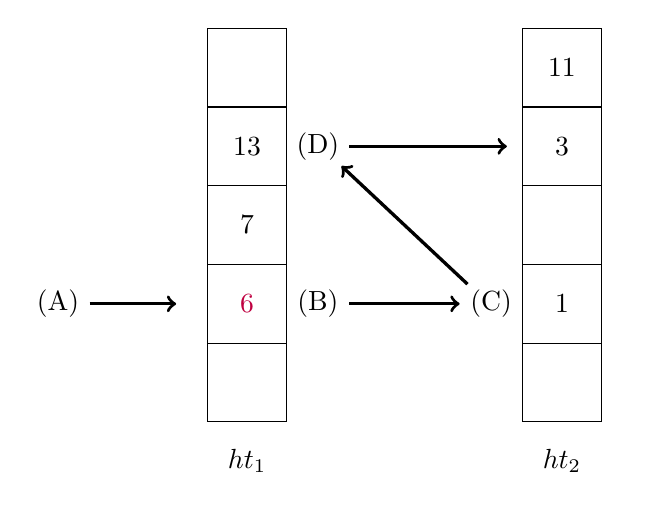
\begin{tikzpicture}[scale=1]
	\foreach \x in {1,2,3,4,5} {
		\tikzmath{int \y; \y=\x-1;}
		\draw (0,\x) rectangle (1,\x+1);
		\node at (-0.2,\x+0.5) {\scriptsize \y};
		\draw (4,\x) rectangle (5,\x+1);
		\node at (5.2,\x+0.5) {\scriptsize \y};
	}
	\node at (0.5,0.5) {\(ht_{1}\)};
	\node at (4.5,0.5) {\(ht_{2}\)};
	\node at (0.5,2.5) {\color{purple}6};
	\node at (0.5,3.5) {7};
	\node at (0.5,4.5) {13};
	\node at (4.5,5.5) {11};
	\node at (4.5,4.5) {3};
	\node at (4.5,2.5) {1};
	\draw[->, line width=1.2pt] (-1.5,2.5) -- (-.4,2.5);
	\draw[->, line width=1.2pt] (1.8,2.5) -- (3.2,2.5);
	\draw[->, line width=1.2pt] (3.3,2.75) -- (1.7,4.25);
	\draw[->, line width=1.2pt] (1.8,4.5) -- (3.8,4.5);
	\node at (-1.9,2.5) {(A)};
	\node at (1.4,2.5) {(B)};
	\node at (3.6,2.5) {(C)};
	\node at (1.4,4.5) {(D)};
	\end{tikzpicture}
	\caption{\(ht_{1}\) und \(ht_{2}\) nach dem Einfügen des Schlüssels 6}
	\label{cuckoo_bsp_4}
\end{figure}

